\chapter{Methodology}
 \section{SOFTWARE DEVELOPMENT APPROACH}
Prototype model is a software development model where instead of freezing the
requirements before design or coding can proceed, a throwaway prototype is built to
understand the requirements. The prototype are usually not complete systems and many
of the details are not built in the prototype. The goal is to provide a system with overall
functionality. In this model, we create the prototype of the actual system, update the
requirements and again rebuild the system until the final requirements are met.
       
 \begin{figure}[hbt]
            \centering
                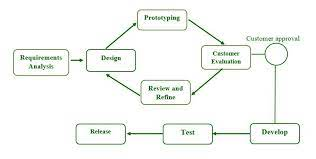
\includegraphics[width=0.75\textwidth]{Images/softwarereq.jpg}
                \caption{Prototype Model for Software Development}
        \end{figure}
    
        \section{ALGORITHMS AND MODELS}
        
Facial recognition systems rely on various algorithms and models to accurately identify and verify individuals based on facial features. Here are some common algorithms and models used in facial recognition systems:

\subsection{Haar Cascades}
\begin{enumerate}
    \item Description: Haar Cascades is an object detection algorithm used for identifying faces in images or video streams. It works by training on positive and negative images to create a classifier.
\item Application: Initial face detection before more detailed analysis.
\end{enumerate}

 \subsection{Local Binary Patterns }
   \begin{itemize}
           \item Description: LBP is a texture descriptor that is often used for facial feature extraction. It focuses on local patterns of pixel intensities.
\item Application: Feature extraction in facial recognition systems.

   \end{itemize}



\subsection{Eigenfaces}
\begin{enumerate}
    \item Description: Eigenfaces is a facial recognition algorithm that uses Principal Component Analysis  to represent facial features in a lower-dimensional space
\item Application: Recognizing faces based on principal components.
\end{enumerate}.

\subsection{Local Feature Analysis }
\begin{enumerate}
    \item Description: LFA focuses on extracting local features, considering facial regions independently. It enhances robustness against variations.
    \item Application: Effective in handling facial variations due to expressions, pose, and lighting.
\end{enumerate}

\subsection{Convolutional Neural Networks}
\begin{enumerate}
    \item Description: CNNs are deep learning models that automatically learn hierarchical features from raw pixel data. They excel at capturing spatial hierarchies in images.
\item Application: State-of-the-art facial recognition, especially when dealing with large datasets and complex variations.
\end{enumerate}

\section{Proposed System}
This system will be able to detect student or employee without physical contact and update the database based on the response from system.
The  system  architecture  of  the  proposed  system  is  given below, 
\newline

\begin[ht]{figure}
    \centering
    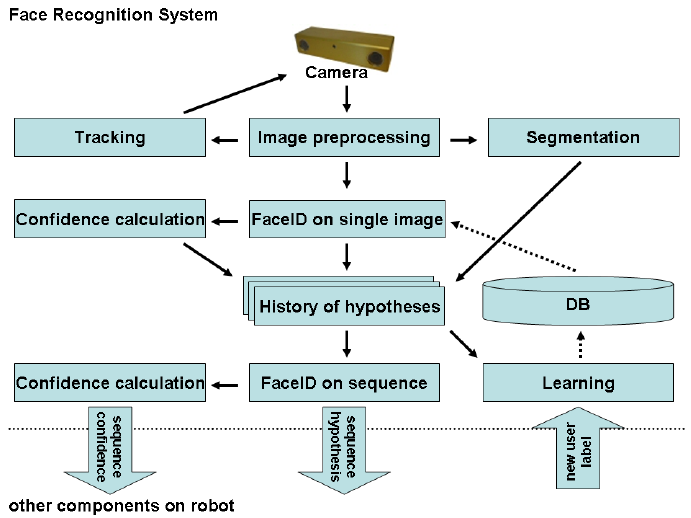
\includegraphics[width=0.75\textwidth]{Images/System-architecture-of-the-face-recognition-system (1).png}
    \caption{Caption}
    \label{fig:enter-label}
\end{figure}

  \subsection{Dataset Creation and Image Preprocessing}
  
 Images of Employee or student are captured using a web cam. Multiple images of single student will be acquired with varied gestures and  angles.  These  images  undergo  pre-processing.  The images  are cropped  to obtain  the  Region of  Interest (ROI) which will be further used in recognition process. Then these  images  will  be  converted  from  RGB  to  gray  scale images. This is done using OpenCV. 
\begin{enumerate}
    \item Step1: we need to read the image with OpenCV’s imread() function:
    \\
  \emph{img = cv2.imread(imagePath)} \\
    This will load the image from the specified file path and return it in the form of a Numpy array. \\
   \emph{img.shape} \\
    Output:\\
    (1000,500,4)
    \item Step2: Convert the RGB data of Image into Greyscale
    To improve computational efficiency, we first need to convert this image to grayscale before performing face detection on it:
    Code \\
   \emph{gray\_image = cv2.cvtColor(img, cv2.COLORBGR2\_GRAY)} 
    Output:
    \\
    (1000,500)\\
    This array only has two values since the image is grayscale and no longer has the third color channel.
\end{enumerate}

  \subsection{Face Detection}
  The idea behind this technique involves using a cascade of classifiers to detect different features in an image. Haar Cascade algorithm needs to be trained to  detect human  faces before it can be used for  face detection. This is called feature extraction. The haar cascade training  data  used  is  an  xml  file- haarcascade\_frontalface\_default. We are using a file called \verb|haarcascade_frontalface_default.xml|. This classifier is designed specifically for detecting frontal faces in visual input.
  \\
)
   \emph{   face\_classifier = cv2.CascadeClassifier(cv2.data.haarcascades + "haarcascade\_frontalface\_default.xml")}
\\
  We are using detectMultiScale module from OpenCV. This is required to create a rectangle around  the faces  in an image.  It has got three  parameters to  consider-  scaleFactor, minNeighbors, minSize.

\subsection{Face Recognition and Calculation}
 Face recognizer  used  in  this  system  is  Local  Binary  Pattern Histogram. Initially, the list of local binary patterns (LBP) of entire  face  is  obtained.  These  LBPs  are  converted  into decimal  number  and  then  histograms  of  all  those  decimal values are made.  At the  end, one  histogram will  be formed for each images in the training data. Later, during recognition process histogram  of the  face to  be recognized  is calculated and then compared with the already computed histograms and returns the  best matched label associated .

 \subsection{DataBase}
 After face recogition process,Based on Calculated histogram Databases are updated .The name of employee or student along with day and time of
attendance is also be stored in the database.
